%%%%%%%%%%%%%%%%%%%%%%%%%%%%%%%%%%%%%%%%%%%%%%%%%%%%%%%%%%%%%%%%%%%%%%%%%% % %
%
% Chapter: Results and Conclusions
% Experimental and/or Theoretical Results demonstrating/proving your solution 
% This section should thoroughly describe the results you obtained. Whenever 
% possible or appropriate, you should try to present your results pictorially 
% using graphs or histograms. In addition you must explain your results; tell 
% the reader what all these data mean.
% Explain the tests you performed (and why)
% Explain how you gathered the data and describe the environment in which you 
% gathered data (include description of any simplifying assumptions you made, 
% any software you wrote or used to run your experiments)
% Present your results. Choose quality over quantity; the reader will not be 
% impressed with pages and pages of graphs and tables, instead s/he wants to 
% be convinced that your results show something interesting and that your 
% experiments support your conclusions.
% Discuss your results! Explain and interpret your results (possibly compare 
% your results to related work). Do not just present data and leave it up to 
% the reader to infer what the data show and why they are interesting. 
% Negative results are interesting too; don't try to hide bad results, but 
% do try to explain them.
%
%%%%%%%%%%%%%%%%%%%%%%%%%%%%%%%%%%%%%%%%%%%%%%%%%%%%%%%%%%%%%%%%%%%%%%%%%%%%%%
 
\chapter{Experimental Results and Analysis: MySQL, MapReduce, and Hive Performance Comparison} \label{ch:results}
This chapter details the RDBMS and DDMS performance comparison experiment using our solutions to the payment history analysis case study. For each solution, we discuss the efficiency and scalability, along with the resulting implications for SMB data management. Our goal was to determine at what point Hadoop and Hive would out-perform MySQL.

The experiment was conducted on the Boise State University Onyx cluster. The cluster configuration and detailed hardware specifications are provided in Appendix~\ref{app:cluster-config}. The experiment was executed sequentially to ensure exclusive access to the server and cluster resources and to avoid the overhead of parallel task execution. Before each execution, we ensured that all nodes were alive and that the integrity of the data was unaltered. Each of the run-times reported reflects the average of three program executions.

\section{Setup}
To provide a fair and controlled environment for our benchmark analysis, we needed to ensure that the computing power of the distributed systems running Hadoop and Hive were comparable to the system running MySQL. 

We installed MySQL on the master node (node00) of the Onyx cluster which is a 4-core hyper-threaded processor, yielding a total of 8 processing threads. We installed the version 5.1.48 (x86\_64) of the MySQL Community Server release for redhat-linux-gnu on the master node of Onyx. The system was configured to use 16GB for the max allowed packet size and 16MB for the net buffer length. We deleted the tables and reloaded the data for each experiment to ensure that the queries were not stored in memory.

We installed Hadoop version 0.20.2 running on Java 1.6.0\_21 which includes both the HDFS and Mapreduce in both pseudo-distributed and distributed configurations. First, we configured the HDFS namenode and MapReduce JobTracker on the Onyx master node (the same as the MySQL server) along with 4 compute nodes as HDFS datanodes and MapReduce TaskTrackers-- also yielding a total of 8 processing threads. Note that since the purpose of the namenode is to maintain the filesystem tree, the metadata for directories in the tree, and the datanode on which all the blocks for a given file are located~\cite{white}, it does not add computing power for MapReduce or Hive in this experiment. We set the number of map tasks per job (\textit{mapred.map.tasks}) to 8, which is 1 task per core. The maximum number of map and reduce tasks are set to 16 and 17, respectively. We left the default replication factor of 3 per block, without compression. Data for both the namenode and datanodes are stored on an \texttt{ext4} directory of the local filesystem. Then, to test Hadoop on the exact same hardware as MySQL, we configured Hadoop to run in pseudo-distributed mode on the master node. In pseudo-distributed mode, each Hadoop daemon runs in a separate Java process. After each benchmark test, we destroy and reformat the HDFS to ensure the uniform distribution of data across nodes. 

We installed Hive version 0.7.0 and configured it to run on top of the same HDFS instance described above. To increase performance, we cluster the tables by primary key into buckets and store data in row format.

\section{Execution}
To determine how well each approach scales as the amount of data increases, we executed the performance benchmark on small (200MB to 500MB), medium (1GB to 5GB), and large (5GB to 10GB) data set sizes. Thus, we varied the number of accounts in the payment analysis data set from 500 to 20,000 records. Each trial was executed from a single client on the master node.

We implemented a performance benchmark test suite using bash shell scripting to help automate the execution process. The suite includes a performance benchmark executable for each of the three solutions that perform the steps enumerated below.

\begin{itemize}
 \item \textbf{MySQL}-- (1) load payment schema to MySQL database, (2) extract data from HDFS using FUSE-DFS module and load to MySQL database tables, (3) execute payment history analysis query, and (4) append query run-time to performance result file.
 \item \textbf{MapReduce}-- (1) ensure HDFS status, (2) execute payment history analysis program, and (3) append program run-time to performance result file.
 \item \textbf{Hive}-- (1) load payment schema to Hive database, (2) load data from HDFS to the Hive database, (3) execute HiveQL payment history analysis query, and (4) append query run-time to performance result file.
\end{itemize}

The suite also includes a script to sequentially run all of the above test scripts for each each trial size, where the experiment procedure is as follows:
\begin{enumerate}
 \item Generate the test data set using \texttt{AccountGen} for the given trial size and record the size of the data set in the performance result file. (On first run, this also involves executing \texttt{HistogramGen} to input for \texttt{AccountGen}).
 \item Execute the MapReduce performance benchmark.
 \item Execute the MySQL performance benchmark.
 \item Execute the Hive performance benchmark.
\end{enumerate}

\section{Results}
Since we chose to generate data based on the number of accounts, we provide the approximate size of the generated data set, namely the \textit{trial size}, for each number of accounts used in our experiments in Table~\ref{tbl:datasetsize}. The approximate sizes are an average of generated data from each of the three trial runs.

 \begin{table}[ht]
  \caption{ Approximate trial size of data set for number of Account records }
  \label{tbl:datasetsize}
  \centerline{
  \small
  \begin{tabular}{|l|l|}
   \hline
   \# Accounts & Approximate trial size\\[0.5ex]
   \hline\hline
   500 & 235 MB\\
   \hline
   1000 & 475 MB\\
   \hline
   2500 & 1 GB\\
   \hline
   5000 & 2 GB\\
   \hline
   10000 & 5 GB\\
   \hline
   15000 & 7 GB\\
   \hline
   20000 & 9 GB\\
   \hline
  \end{tabular}
  }
 \end{table}

Figure~\ref{fig:allruntimes} and Table~\ref{tbl:results} display the performance results of MySQL, MapReduce and Hive for each trial size with the MySQL server running on the master node of the onyx cluster and the Hadoop namenode running on the master node of the Onyx cluster and four data nodes running on four compute nodes.  

 \begin{table}[ht]
  \caption{Run-time (seconds) performance of MySQL server running on master node and MapReduce / Hive running on master node plus four data nodes}
  \label{tbl:results}
  \centerline{
  \small
  \begin{tabular}{|l||l|l|l|}
   \hline
   \# Accounts& MySQL & MapReduce & Hive\\[0.5ex]
   \hline\hline
   500 & 4.20 & 81.14 & 535.1\\
   \hline
   1000 & 13.83 & 82.55 & 543.64\\
   \hline
   2500 & 85.42 & 84.41 & 548.45\\
   \hline
   5000 & 392.42 & 83.42 & 553.44\\
   \hline
   10000 & 1518.18 & 88.14 & 557.51\\
   \hline
   15000 & 1390.25 & 86.85 & 581.5\\
   \hline
   20000 & 2367.81 & 88.90 & 582.7\\
   \hline
  \end{tabular}
  }
 \end{table}

\begin{figure}[h!]
 \centering
 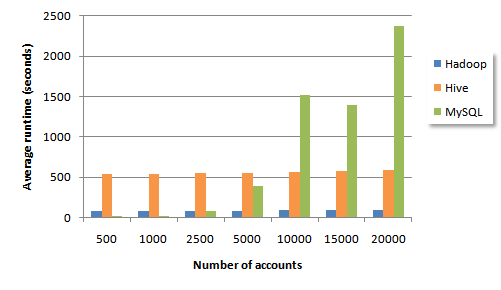
\includegraphics[width=\textwidth]{../images/runtime_vs_accountCount.png}
 % graph-all-runtimes.eps: 0x0 pixel, 300dpi, 0.00x0.00 cm, bb=14 14 630 433
 \caption{Run-time (seconds) performance of MySQL server running on master node and MapReduce / Hive running on master node plus four data nodes}
 \label{fig:allruntimes}
\end{figure}

Figure~\ref{fig:allruntimespseudo} and Table~\ref{tbl:resultspseudo} display the performance results of MySQL, MapReduce and Hive for each trial size with MySQL server running on the master node of the Onyx cluster and Hadoop running in pseudo-distributed mode on the master node of the Onyx cluster.  

 \begin{table}[ht]
  \caption{Run-time (seconds) performance of MySQL server running on master node and MapReduce / Hive running in pseudo-distributed mode}
  \label{tbl:resultspseudo}
  \centerline{
  \small
  \begin{tabular}{|l||l|l|l|}
   \hline
   \# Accounts& MySQL & MapReduce & Hive\\[0.5ex]
   \hline\hline
   500 & 4.20 & 79.45 & 532.01\\
   \hline
   1000 & 13.83 & 79.50 & 531.55\\
   \hline
   2500 & 85.42 & 79.42 & 534.16\\
   \hline
   5000 & 392.42 & 79.44 & 537.00\\
   \hline
   10000 & 1518.18 & 81.48 & 543.51\\
   \hline
   15000 & 1390.25 & 82.39 & 543.95\\
   \hline
   20000 & 2367.81 & 87.47 & 543.64\\
   \hline
  \end{tabular}
  }
 \end{table}

\begin{figure}[h!]
 \centering
 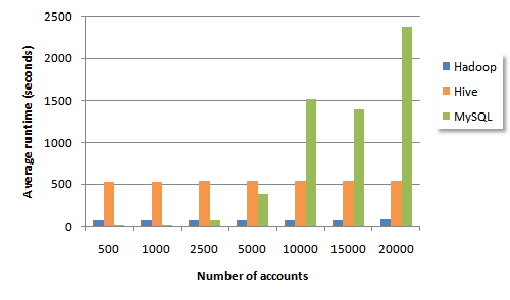
\includegraphics[width=\textwidth]{../images/runtime_vs_accountCount_pseudoDistributed.png}
 % graph-all-runtimes.eps: 0x0 pixel, 300dpi, 0.00x0.00 cm, bb=14 14 630 433
 \caption{Run-time (seconds) performance of MySQL server running on master node and MapReduce / Hive running on master node in pseudo-distributed mode}
 \label{fig:allruntimespseudo}
\end{figure}

MySQL outperforms both MapReduce and Hive for trial sizes ranging from 500 to 2,500 accounts. Since the amount of data generated for these trials is relatively small, 235MB to 1GB, the results are as expected. Aside from an anomaly at 15,000 accounts, the run-times continue to increase as expected with the size of the data set. At 15,000 accounts the MySQL run-time decreases from 1518.18 seconds to 1390.25 seconds. The MapReduce run-time also decreases from 88.14 seconds to 86.85 seconds at this same trial size. Since the data is randomly generated and the anomaly occurred for both MySQL and Hive, it may be explained by less complex data in this data range.

In both distributed and pseudo-distributed mode, MapReduce run-times remain steady at in the range of 81 to 90 seconds for all trial sizes, converging and surpassing MySQL performance at around 2,500 accounts. Hive run-times also remain steady in the range of 535 to 583 seconds for all trials, converging and surpassing MySQL performance at around 5,000 accounts. As expected with the relatively small trial sizes, MapReduce and Hive performed better in psuedo-distributed mode than in distributed mode with the same number of processing cores because there is no network communication and the drives are twice as fast. However, as the amount of data increases we expect better performance in distributed mode.

%  \begin{table}[ht]
%   \caption{The average run-times (seconds) per account}
%   \label{tbl:avg-account-runtimes}
%   \centerline{
%   \small
%   \begin{tabular}{|l||l|l|l|}
%    \hline
%    \# Accounts & MySQL & MapReduce & Hive\\[0.5ex]
%    \hline\hline
%    500 & 0.01 & 0.16 & 1.07\\
%    \hline
%    1000 & 0.01 & 0.08 & 0.54\\
%    \hline
%    2500 & 0.03 & 0.03 & 0.22\\
%    \hline
%    5000 & 0.08 & 0.02 & 0.11\\
%    \hline
%    10000 & 0.15 & 0.01 & 0.06\\
%    \hline
%    15000 & 0.09 & 0.01 & 0.04\\
%    \hline
%    20000 & 0.12 & 0 & 0.03\\
%    \hline
%   \end{tabular}
%   }
%  \end{table}
% 
% Table ~\ref{tbl:avg-account-runtimes} displays the solution run-times divided by the trial size. It is evident that performance per account for both MapReduce and Hive improves as the trial size increases, whereas the MySQL performance decreases. 

From these results, it is evident that MapReduce outperforms MySQL and Hive by a dramatic margin. Therefore, for test data sets greater than 1GB, MapReduce emerges as the best candidate solution for the payment history analysis case study provided by CompanyX. Furthermore, we investigate whether we can improve MapReduce performance further by varying the number of map tasks per datanode; Figure ~\ref{fig:maptasks} displays the results for 1, 2, and 4 map tasks per datanode. In this case, we observe that MapReduce with 1 map task per datanode slightly outperforms 2 and 4 map tasks per datanode.

\begin{figure}[h!]
 \centering
 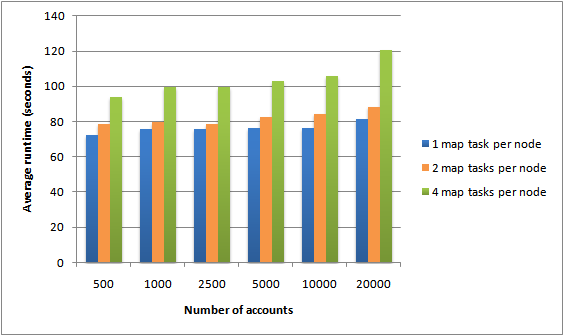
\includegraphics[width=\textwidth]{../images/runtime_vs_mapTasks.png}
 % graph-all-runtimes.eps: 0x0 pixel, 300dpi, 0.00x0.00 cm, bb=14 14 630 433
 \caption{Scalability of MapReduce run-time (seconds) performance for a varied number of map tasks per datanode}
 \label{fig:maptasks}
\end{figure}